\documentclass[10pt,a4paper]{article}

% Packages
\usepackage[utf8]{inputenc}
\usepackage[french]{babel}
\usepackage[T1]{fontenc}
\usepackage[margin=1.35cm]{geometry}
\usepackage{lmodern}
\usepackage{microtype}
\usepackage{graphicx}
\usepackage{float}
\usepackage{hyperref}
\usepackage{xcolor}
\usepackage{booktabs}
\usepackage{caption}
\usepackage{subcaption}
\usepackage{fancyhdr}
\usepackage{titlesec}
\usepackage{multicol}
\usepackage{array}
\usepackage{textcomp}
\usepackage{enumitem}
\usepackage{setspace}

% Configuration
\setlength{\parindent}{0pt}
\setlength{\parskip}{2pt}
\setlength{\textfloatsep}{8pt}
\setlength{\intextsep}{8pt}
\setlength{\abovecaptionskip}{4pt}
\setlength{\belowcaptionskip}{0pt}
\raggedbottom

\pagestyle{fancy}
\fancyhf{}
\fancyhead[L]{\footnotesize Analyse Climatique - Master 2 Big Data}
\fancyhead[R]{\footnotesize Mars 2026}
\fancyfoot[C]{\thepage}
\renewcommand{\headrulewidth}{0.2pt}

\graphicspath{{outputs/}}
\setlist[itemize]{leftmargin=*, nosep}
\setlist[enumerate]{leftmargin=*, nosep}

% Couleurs
\definecolor{titlecolor}{RGB}{0,51,102}
\definecolor{boxcolor}{RGB}{240,240,240}

% Titres
\titleformat{\section}{\normalfont\large\bfseries\color{titlecolor}}{\thesection}{0.3em}{}
\titleformat{\subsection}{\normalfont\normalsize\bfseries\color{titlecolor}}{\thesubsection}{0.3em}{}

% Configuration des captions
\captionsetup{font=footnotesize,labelfont=bf}

\begin{document}

\begin{center}
{\Large\bfseries\color{titlecolor}Rapport Final -- Projet d'Analyse de Données Climatiques\par}
\vspace{0.15cm}
{\normalsize \textbf{SAMSON APIE PAWOUANG}\par}
\vspace{0.15cm}
{\footnotesize Master 2 -- Big Data \quad \textbullet \quad Mars 2026\par}
\end{center}
\vspace{0.3cm}

\section{Introduction}
Ce rapport présente l'analyse de données climatiques réalisée sur le fichier \texttt{GlobalLandTemperaturesByMajorCity.csv}. L'objectif est de démontrer la capacité à manipuler un volume de données conséquent, structurer un traitement et produire une analyse exploitable.

\section{Étape 1 -- Prise en main des données}
\subsection{Structure du jeu de données}

\textbf{Dimensions initiales :}
\begin{itemize}
\item \textbf{Nombre de lignes} : \textasciitilde{}239\,000 lignes
\item \textbf{Nombre de colonnes} : 7 colonnes
\end{itemize}

\textbf{Variables identifiées :}
\begin{table}[H]
\centering
\footnotesize
\begin{tabular}{lll}
\toprule
\textbf{Variable} & \textbf{Type} & \textbf{Description} \\
\midrule
\texttt{dt} & object (date) & Date de la mesure (format YYYY-MM-DD) \\
\texttt{AverageTemperature} & float64 & Température moyenne mensuelle (\textdegree C) \\
\texttt{AverageTemperatureUncertainty} & float64 & Incertitude de mesure \\
\texttt{City} & object & Nom de la ville \\
\texttt{Country} & object & Pays \\
\texttt{Latitude} & object & Latitude (format texte) \\
\texttt{Longitude} & object & Longitude (format texte) \\
\bottomrule
\end{tabular}
\caption{Variables du fichier source}
\end{table}

\subsection{Problèmes identifiés}
\begin{enumerate}
\item \textbf{Valeurs manquantes importantes} : \texttt{AverageTemperature} et \texttt{AverageTemperatureUncertainty} présentent des valeurs manquantes (principalement avant 1850).
\item \textbf{Volume de données} : le volume initial reste important pour une analyse directe.
\item \textbf{Variables inutiles / peu exploitables} : coordonnées géographiques au format texte ; incertitude peu utile pour la classification.
\item \textbf{Période historique très large} : qualité des mesures anciennes potentiellement faible.
\end{enumerate}

\textbf{Conclusion :} le dataset nécessite un nettoyage et une réduction pour être exploitable efficacement.

\begin{figure}[H]
\centering
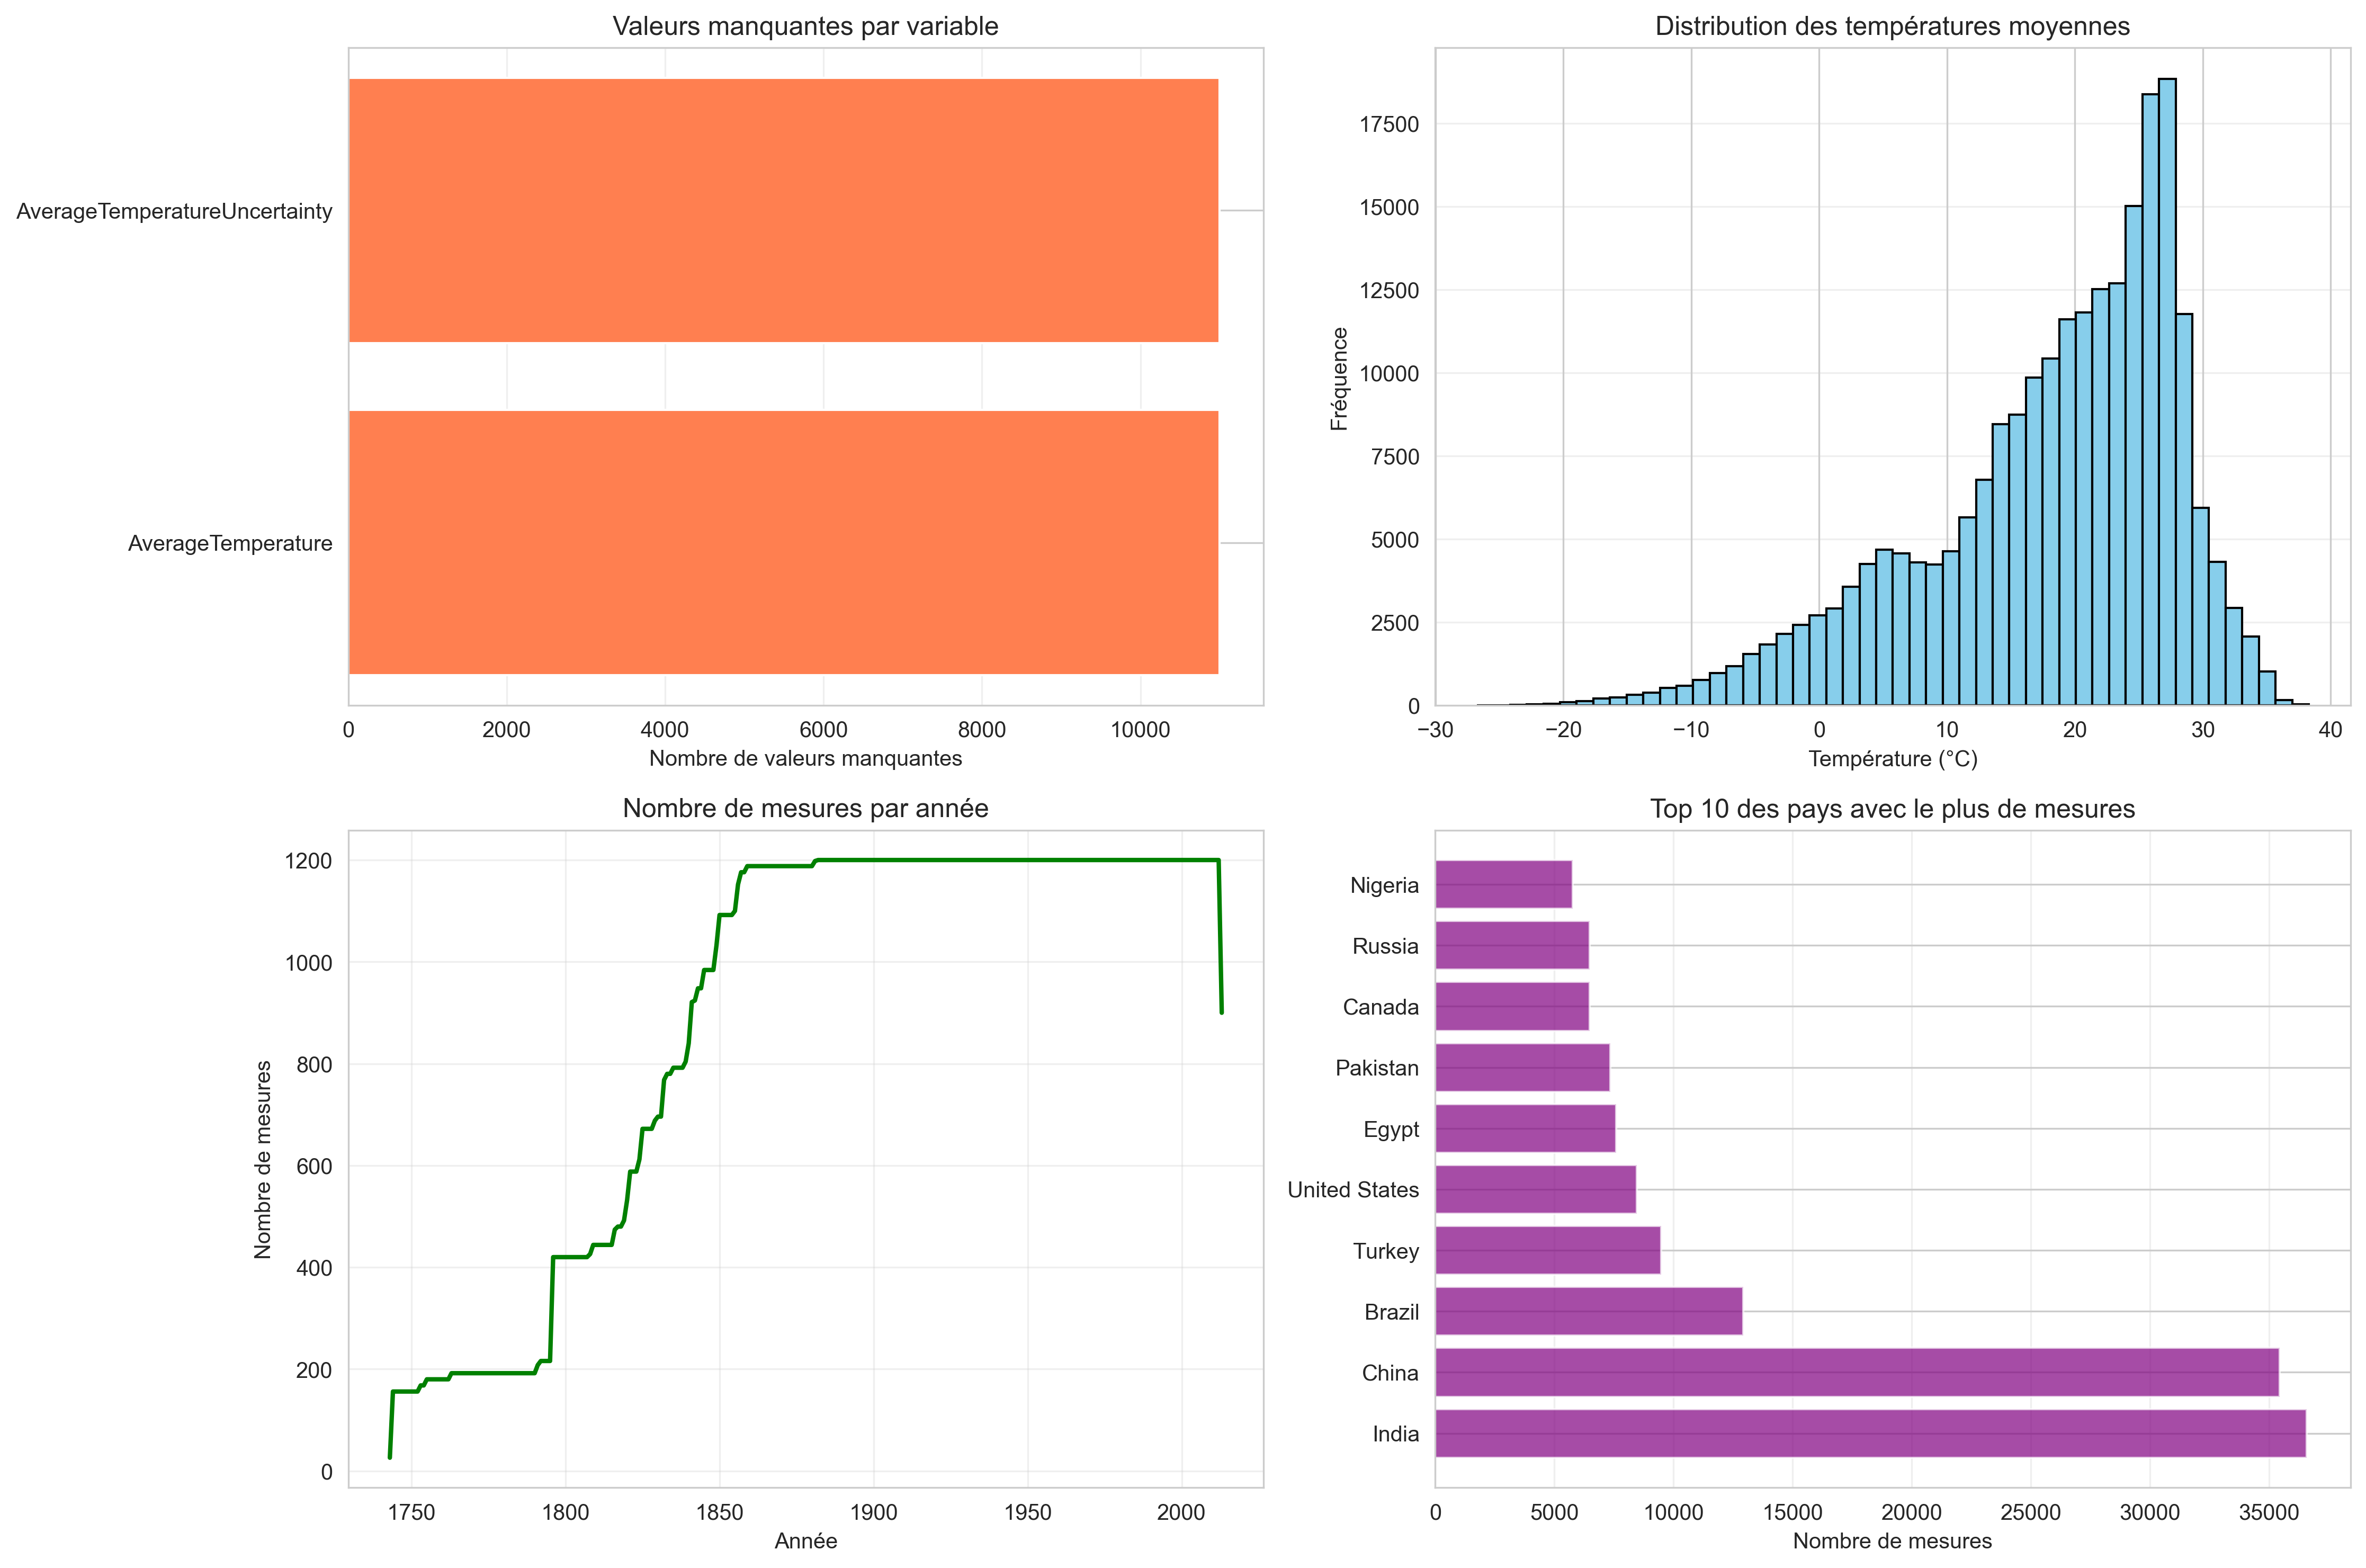
\includegraphics[width=0.90\textwidth]{step1_exploratory_analysis.png}
\caption{Analyse exploratoire (étape 1)}
\end{figure}

\section{Étape 2 -- Réduction du volume de données}
\subsection{Stratégie choisie : filtrage temporel}

\textbf{Approche retenue :} conservation uniquement des données à partir de 1950.

\subsection{Justification}
\begin{enumerate}
  \item \textbf{Qualité des données} : les mesures modernes (post-1950) sont plus fiables.
  \item \textbf{Pertinence métier} : période récente plus adaptée à l'analyse actuelle.
  \item \textbf{Volume suffisant} : le dataset réduit conserve un volume important.
  \item \textbf{Cohérence} : évite les biais liés aux mesures anciennes moins précises.
\end{enumerate}

\subsection{Implémentation}
\footnotesize
\colorbox{boxcolor}{\parbox{0.96\textwidth}{\texttt{dt} convertie en date ; suppression des NA sur \texttt{AverageTemperature} ; filtrage \texttt{Year} \geq 1950 ; sauvegarde en \texttt{dataset\_reduced.csv}.}}
\normalsize

\subsection{Résultat}
\begin{itemize}
  \item \textbf{Après filtrage temporel} : \textbf{\textasciitilde{}76\,400 lignes}
  \item \textbf{Réduction} : 68\% du volume initial
\end{itemize}

\begin{figure}[H]
\centering
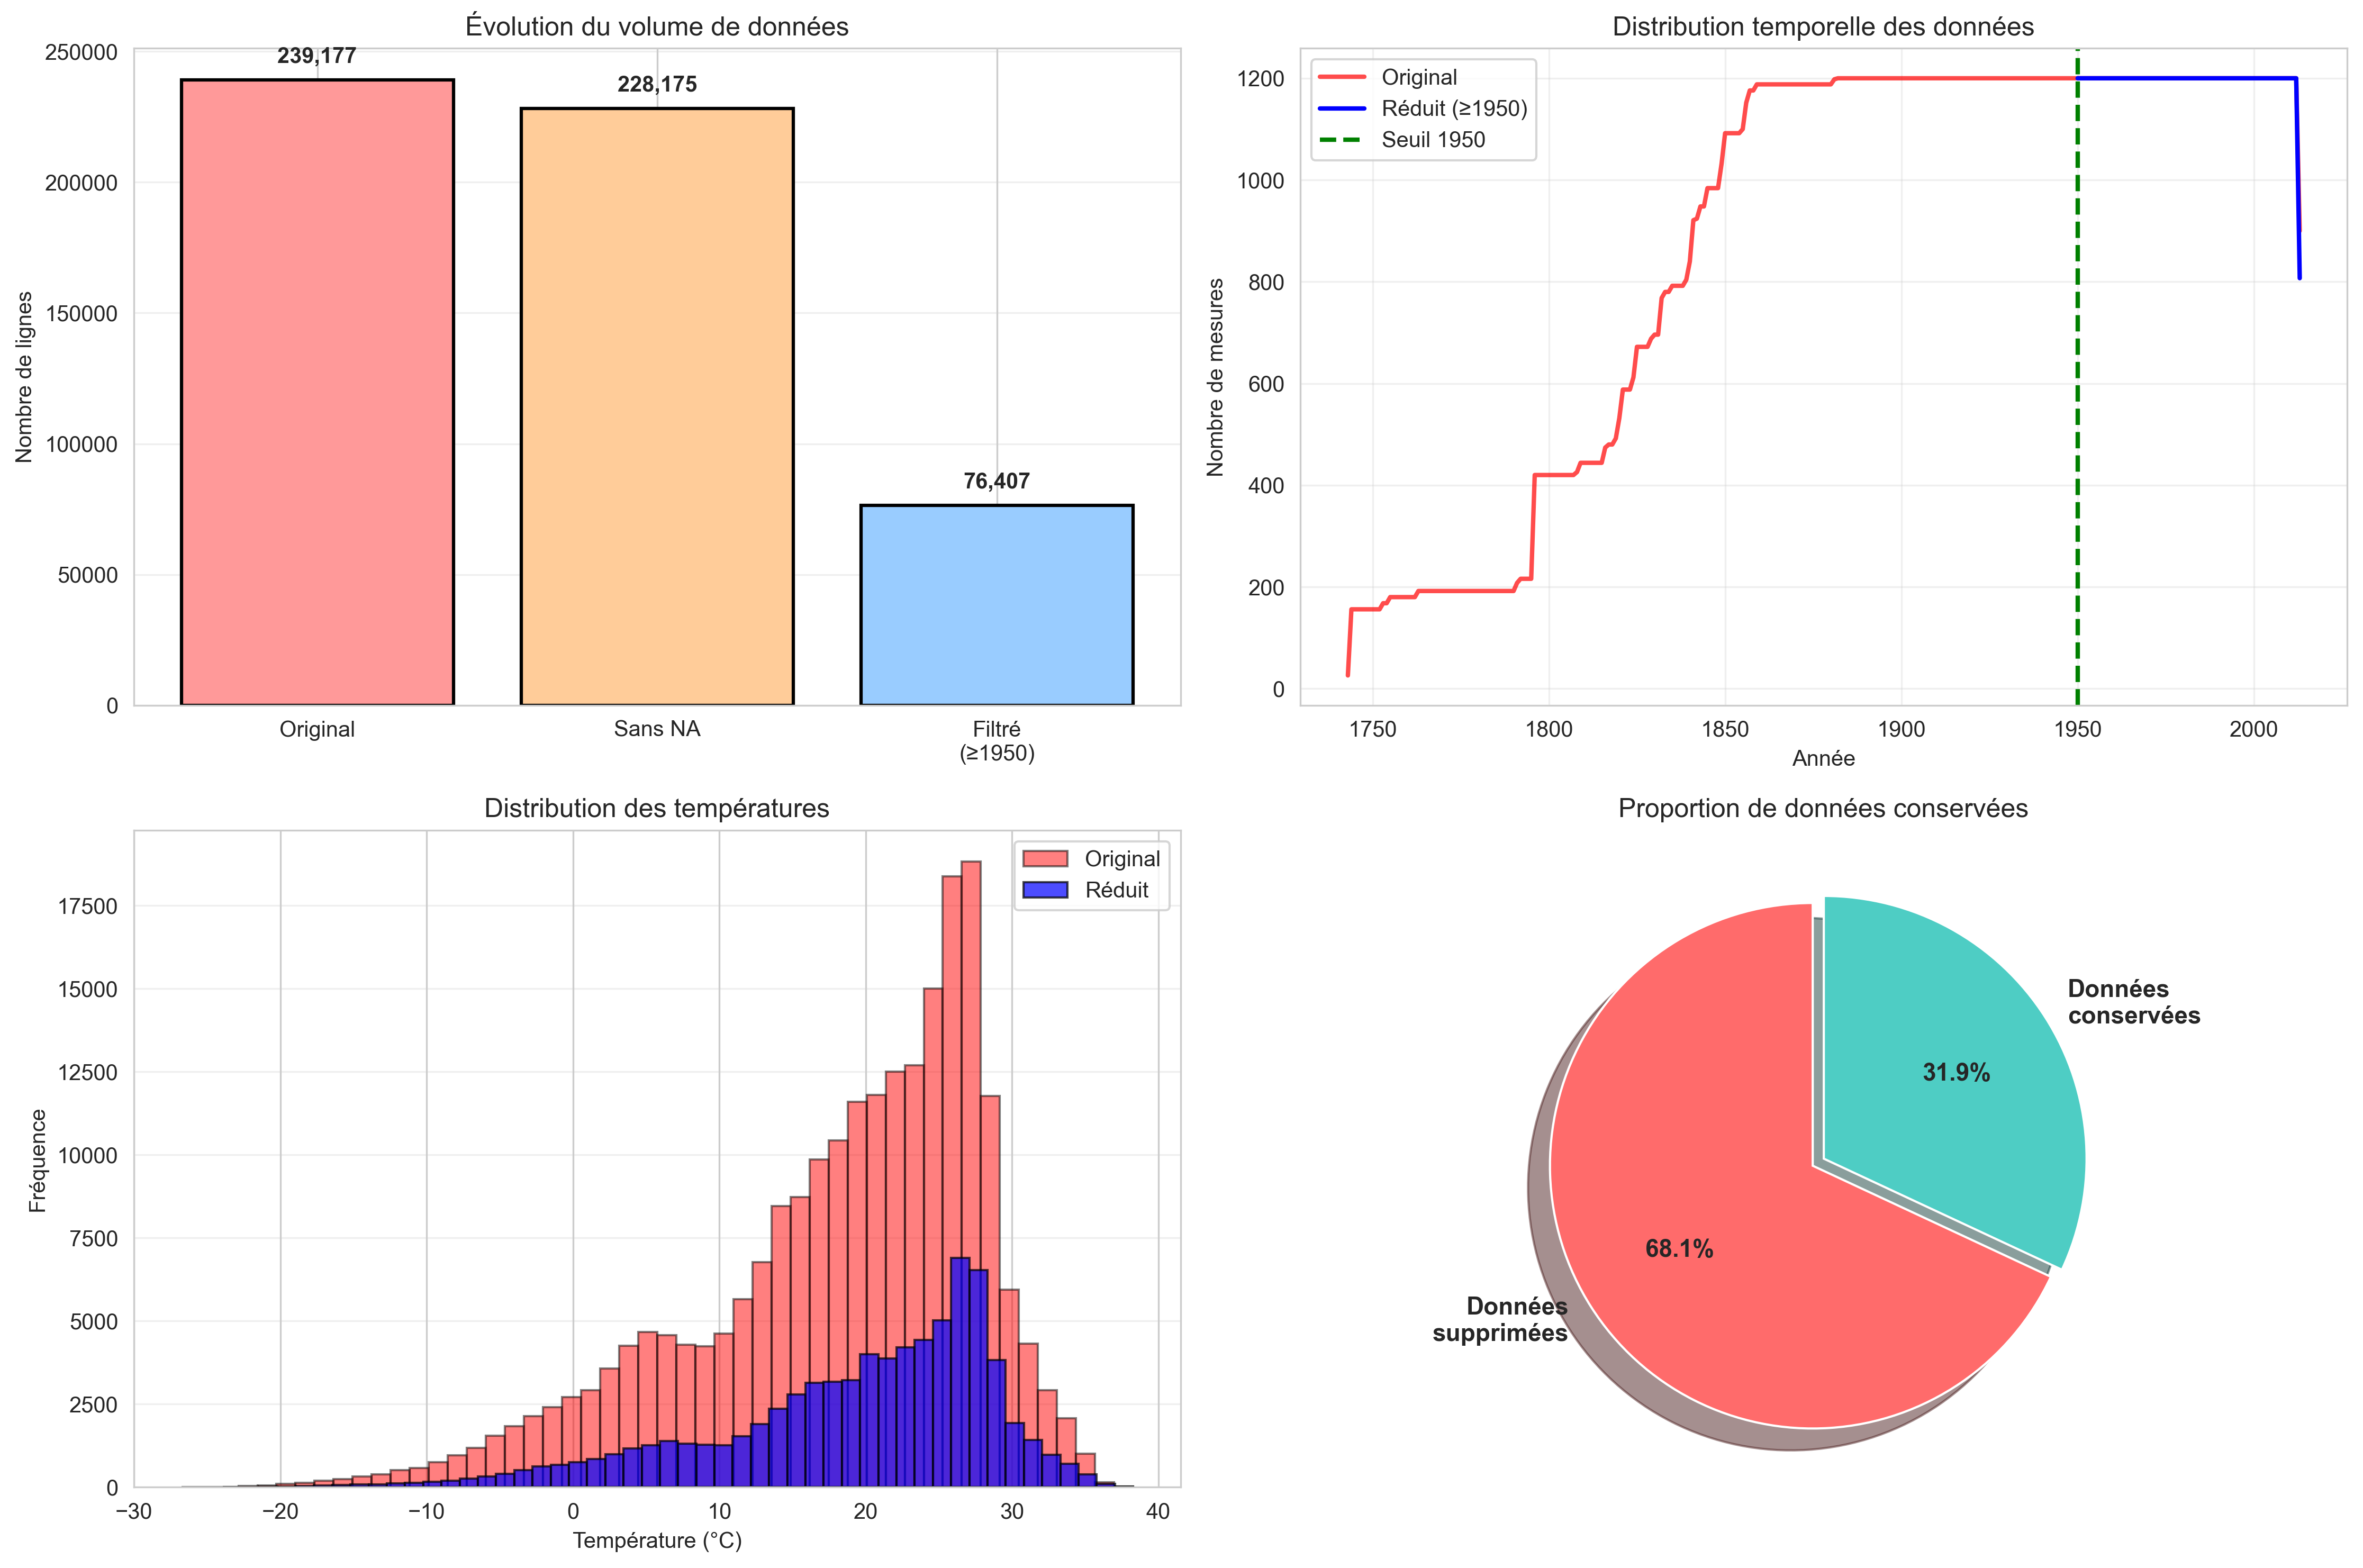
\includegraphics[width=0.90\textwidth]{step2_data_reduction.png}
\caption{Réduction du volume (étape 2)}
\end{figure}

\section{Étape 3 -- Création d'une variable cible}
\subsection{Méthode de classification}

\textbf{Variable créée :} \texttt{temperature\_class}.

\textbf{Approche :} classification basée sur les quantiles.
\begin{itemize}
  \item \textbf{Quantile 33\%} : seuil entre \textit{Basse} et \textit{Moyenne}
  \item \textbf{Quantile 66\%} : seuil entre \textit{Moyenne} et \textit{Élevée}
\end{itemize}

\subsection{Seuils calculés}
\begin{itemize}
  \item \textbf{Seuil 33\%} : 16.95\textdegree C
  \item \textbf{Seuil 66\%} : 25.04\textdegree C
\end{itemize}

\subsection{Classes définies}
\begin{table}[H]
\centering
\footnotesize
\begin{tabular}{lll}
\toprule
\textbf{Classe} & \textbf{Condition} & \textbf{Interprétation} \\
\midrule
Basse & $T \leq 16{,}95$ & Climats froids, mois d'hiver \\
Moyenne & $16{,}95 < T \leq 25{,}04$ & Climats tempérés, intersaisons \\
Élevée & $T > 25{,}04$ & Climats chauds, mois d'été \\
\bottomrule
\end{tabular}
\caption{Définition de \texttt{temperature\_class}}
\end{table}

\subsection{Répartition des classes}
\begin{table}[H]
\centering
\footnotesize
\begin{tabular}{lrr}
\toprule
\textbf{Classe} & \textbf{Nombre d'observations} & \textbf{Proportion} \\
\midrule
Basse & 25\,214 & 33.0\% \\
Moyenne & 25\,217 & 33.0\% \\
Élevée & 25\,976 & 34.0\% \\
\bottomrule
\end{tabular}
\caption{Répartition des classes}
\end{table}

\textbf{Conclusion :} les classes sont équilibrées de manière raisonnable grâce aux quantiles.

\begin{figure}[H]
\centering
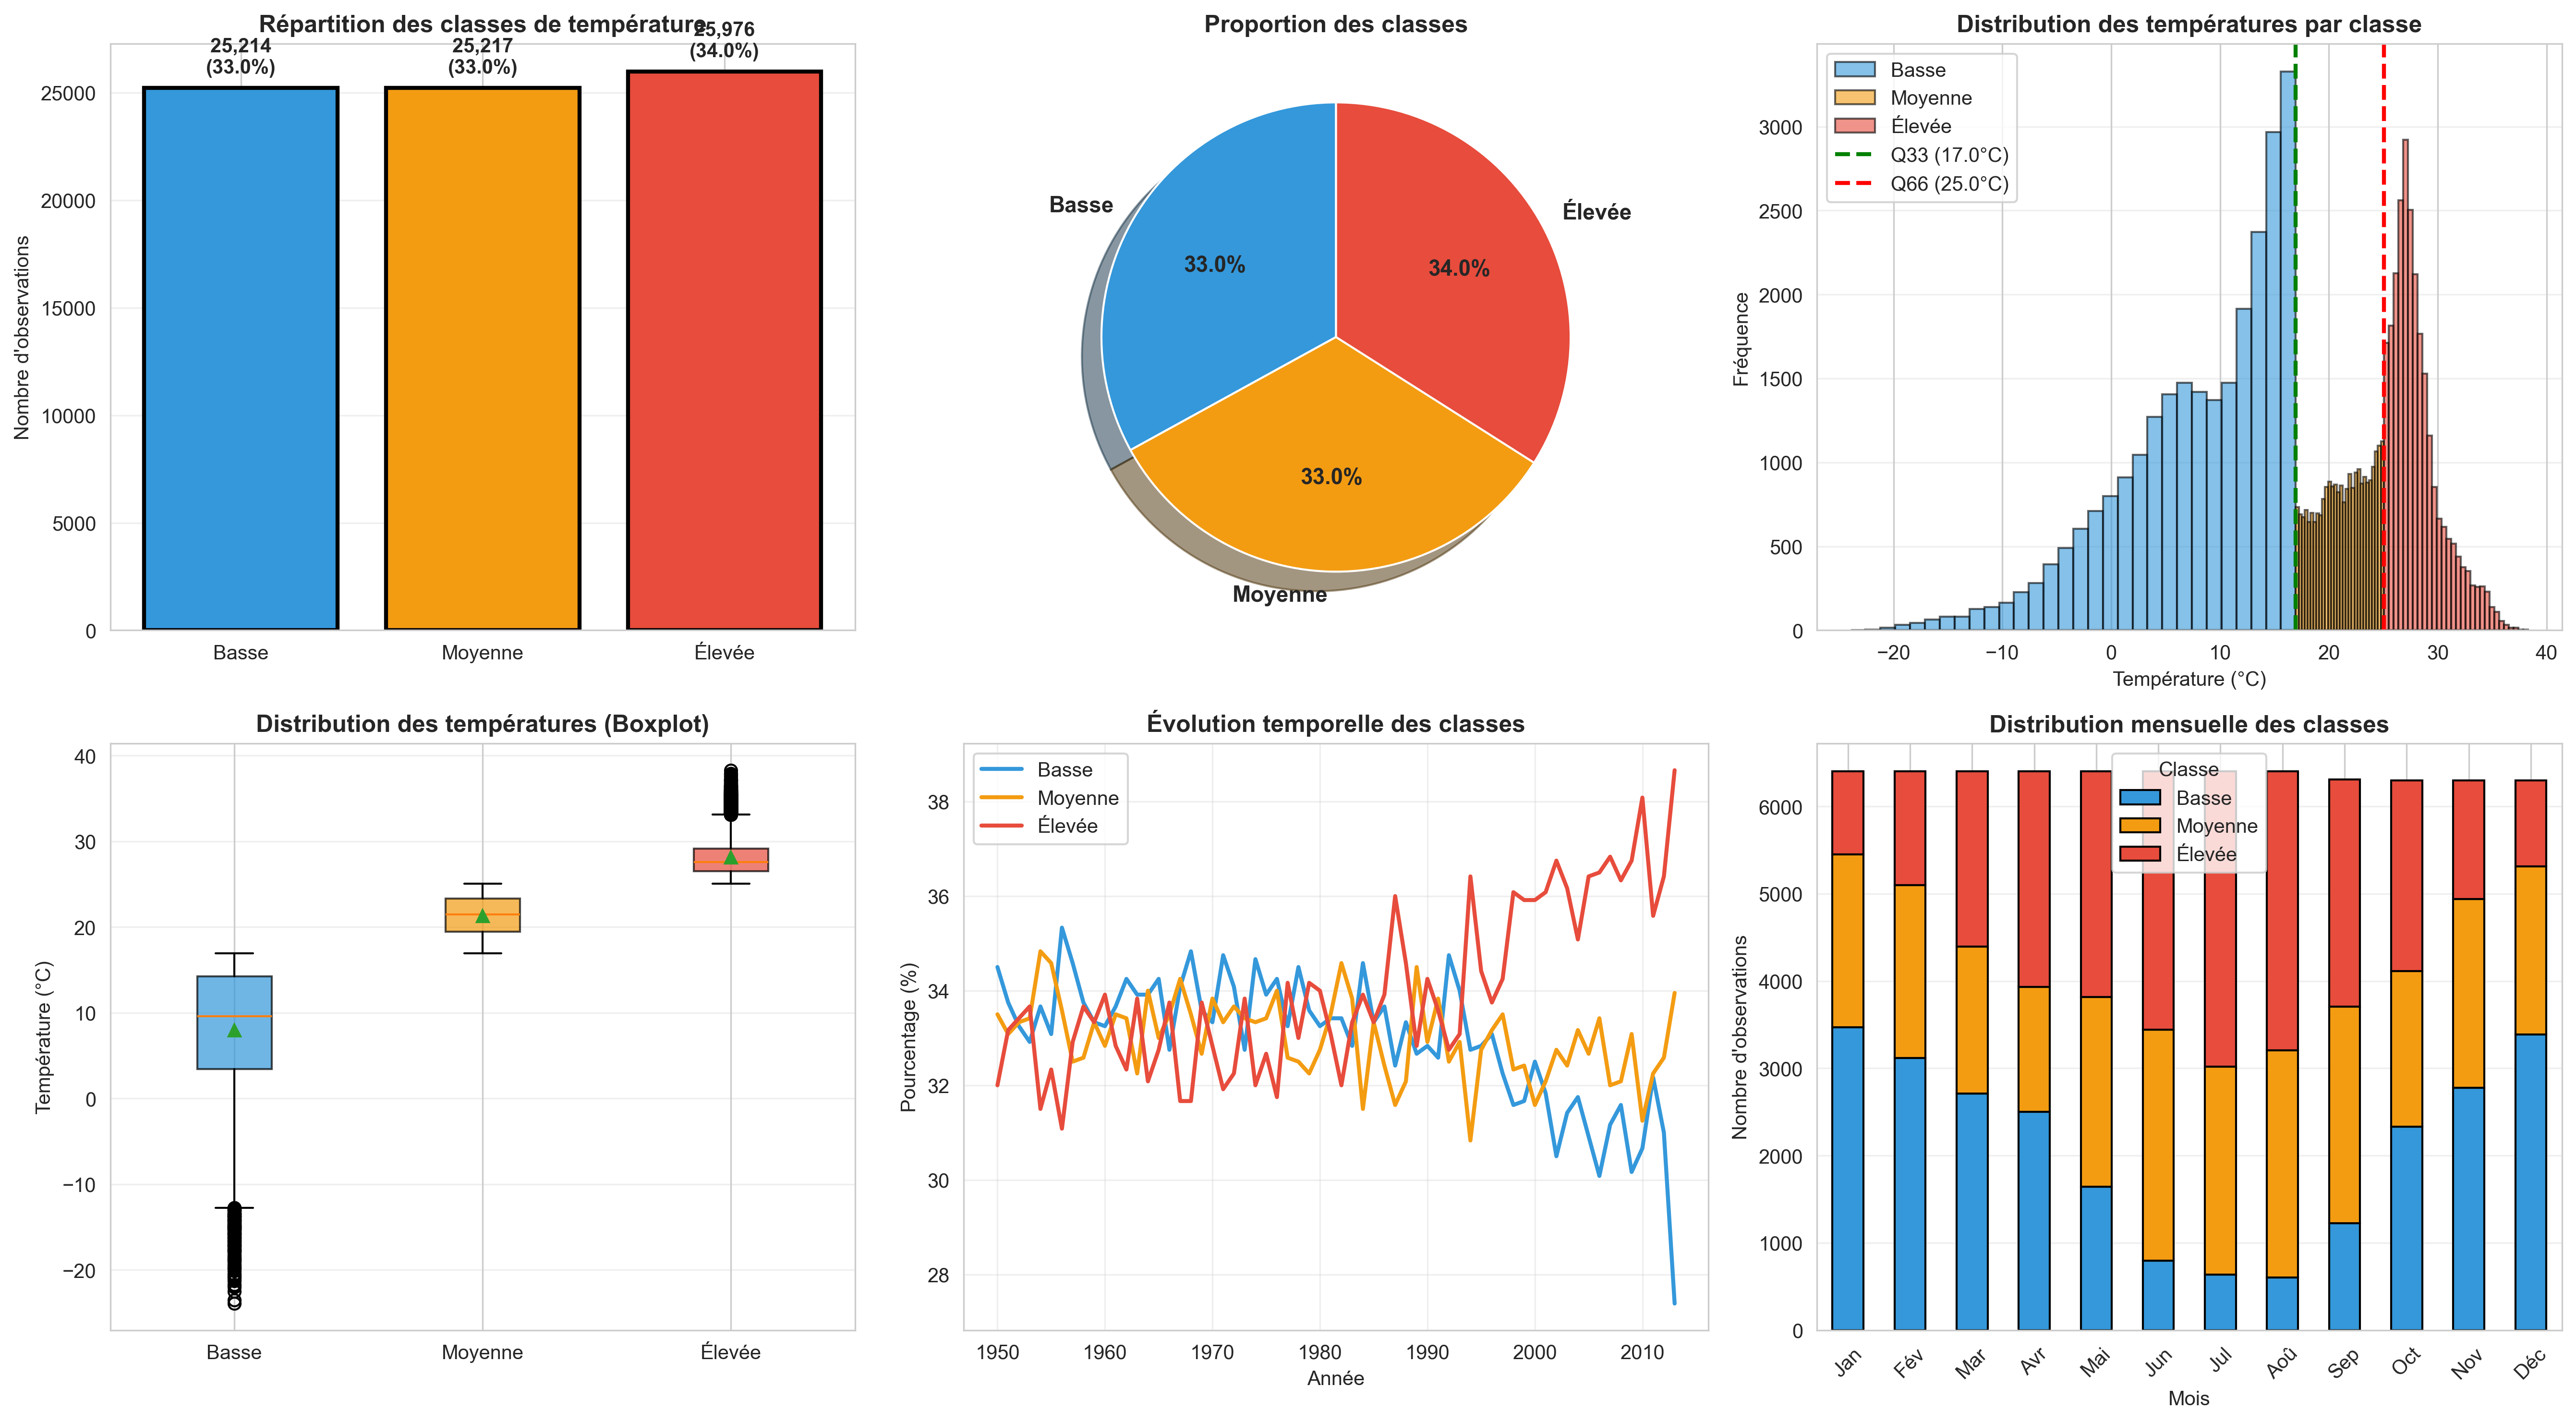
\includegraphics[width=0.90\textwidth]{step3_target_creation.png}
\caption{Création de la cible (étape 3)}
\end{figure}

\section{Étape 4 -- Préparation des données pour Sipina}
\subsection{Variables sélectionnées}

\textbf{Variables explicatives retenues :}
\begin{enumerate}
\item \textbf{City} : nom de la ville
\item \textbf{Country} : pays
\item \textbf{Latitude} : position géographique Nord-Sud (texte)
\item \textbf{Longitude} : position géographique Est-Ouest (texte)
\item \textbf{Year} : année
\item \textbf{Month} : mois (1--12)
\end{enumerate}

\textbf{Variable cible :} \texttt{temperature\_class}.

\subsection{Transformations appliquées}
\begin{enumerate}
\item \textbf{Extraction temporelle} : création de \texttt{Year} et \texttt{Month}.
\item \textbf{Suppression des variables inutiles} : \texttt{dt}, \texttt{AverageTemperature}, \texttt{AverageTemperatureUncertainty}.
\item \textbf{Traitement des valeurs manquantes} : aucune valeur manquante restante après étape 2.
\end{enumerate}

\subsection{Fichier final}
\begin{itemize}
\item \textbf{Nom} : \texttt{dataset\_final\_sipina.csv}
\item \textbf{Dimensions} : 76\,407 lignes $\times$ 7 colonnes
\item \textbf{Encodage} : UTF-8
\end{itemize}

\begin{figure}[H]
\centering
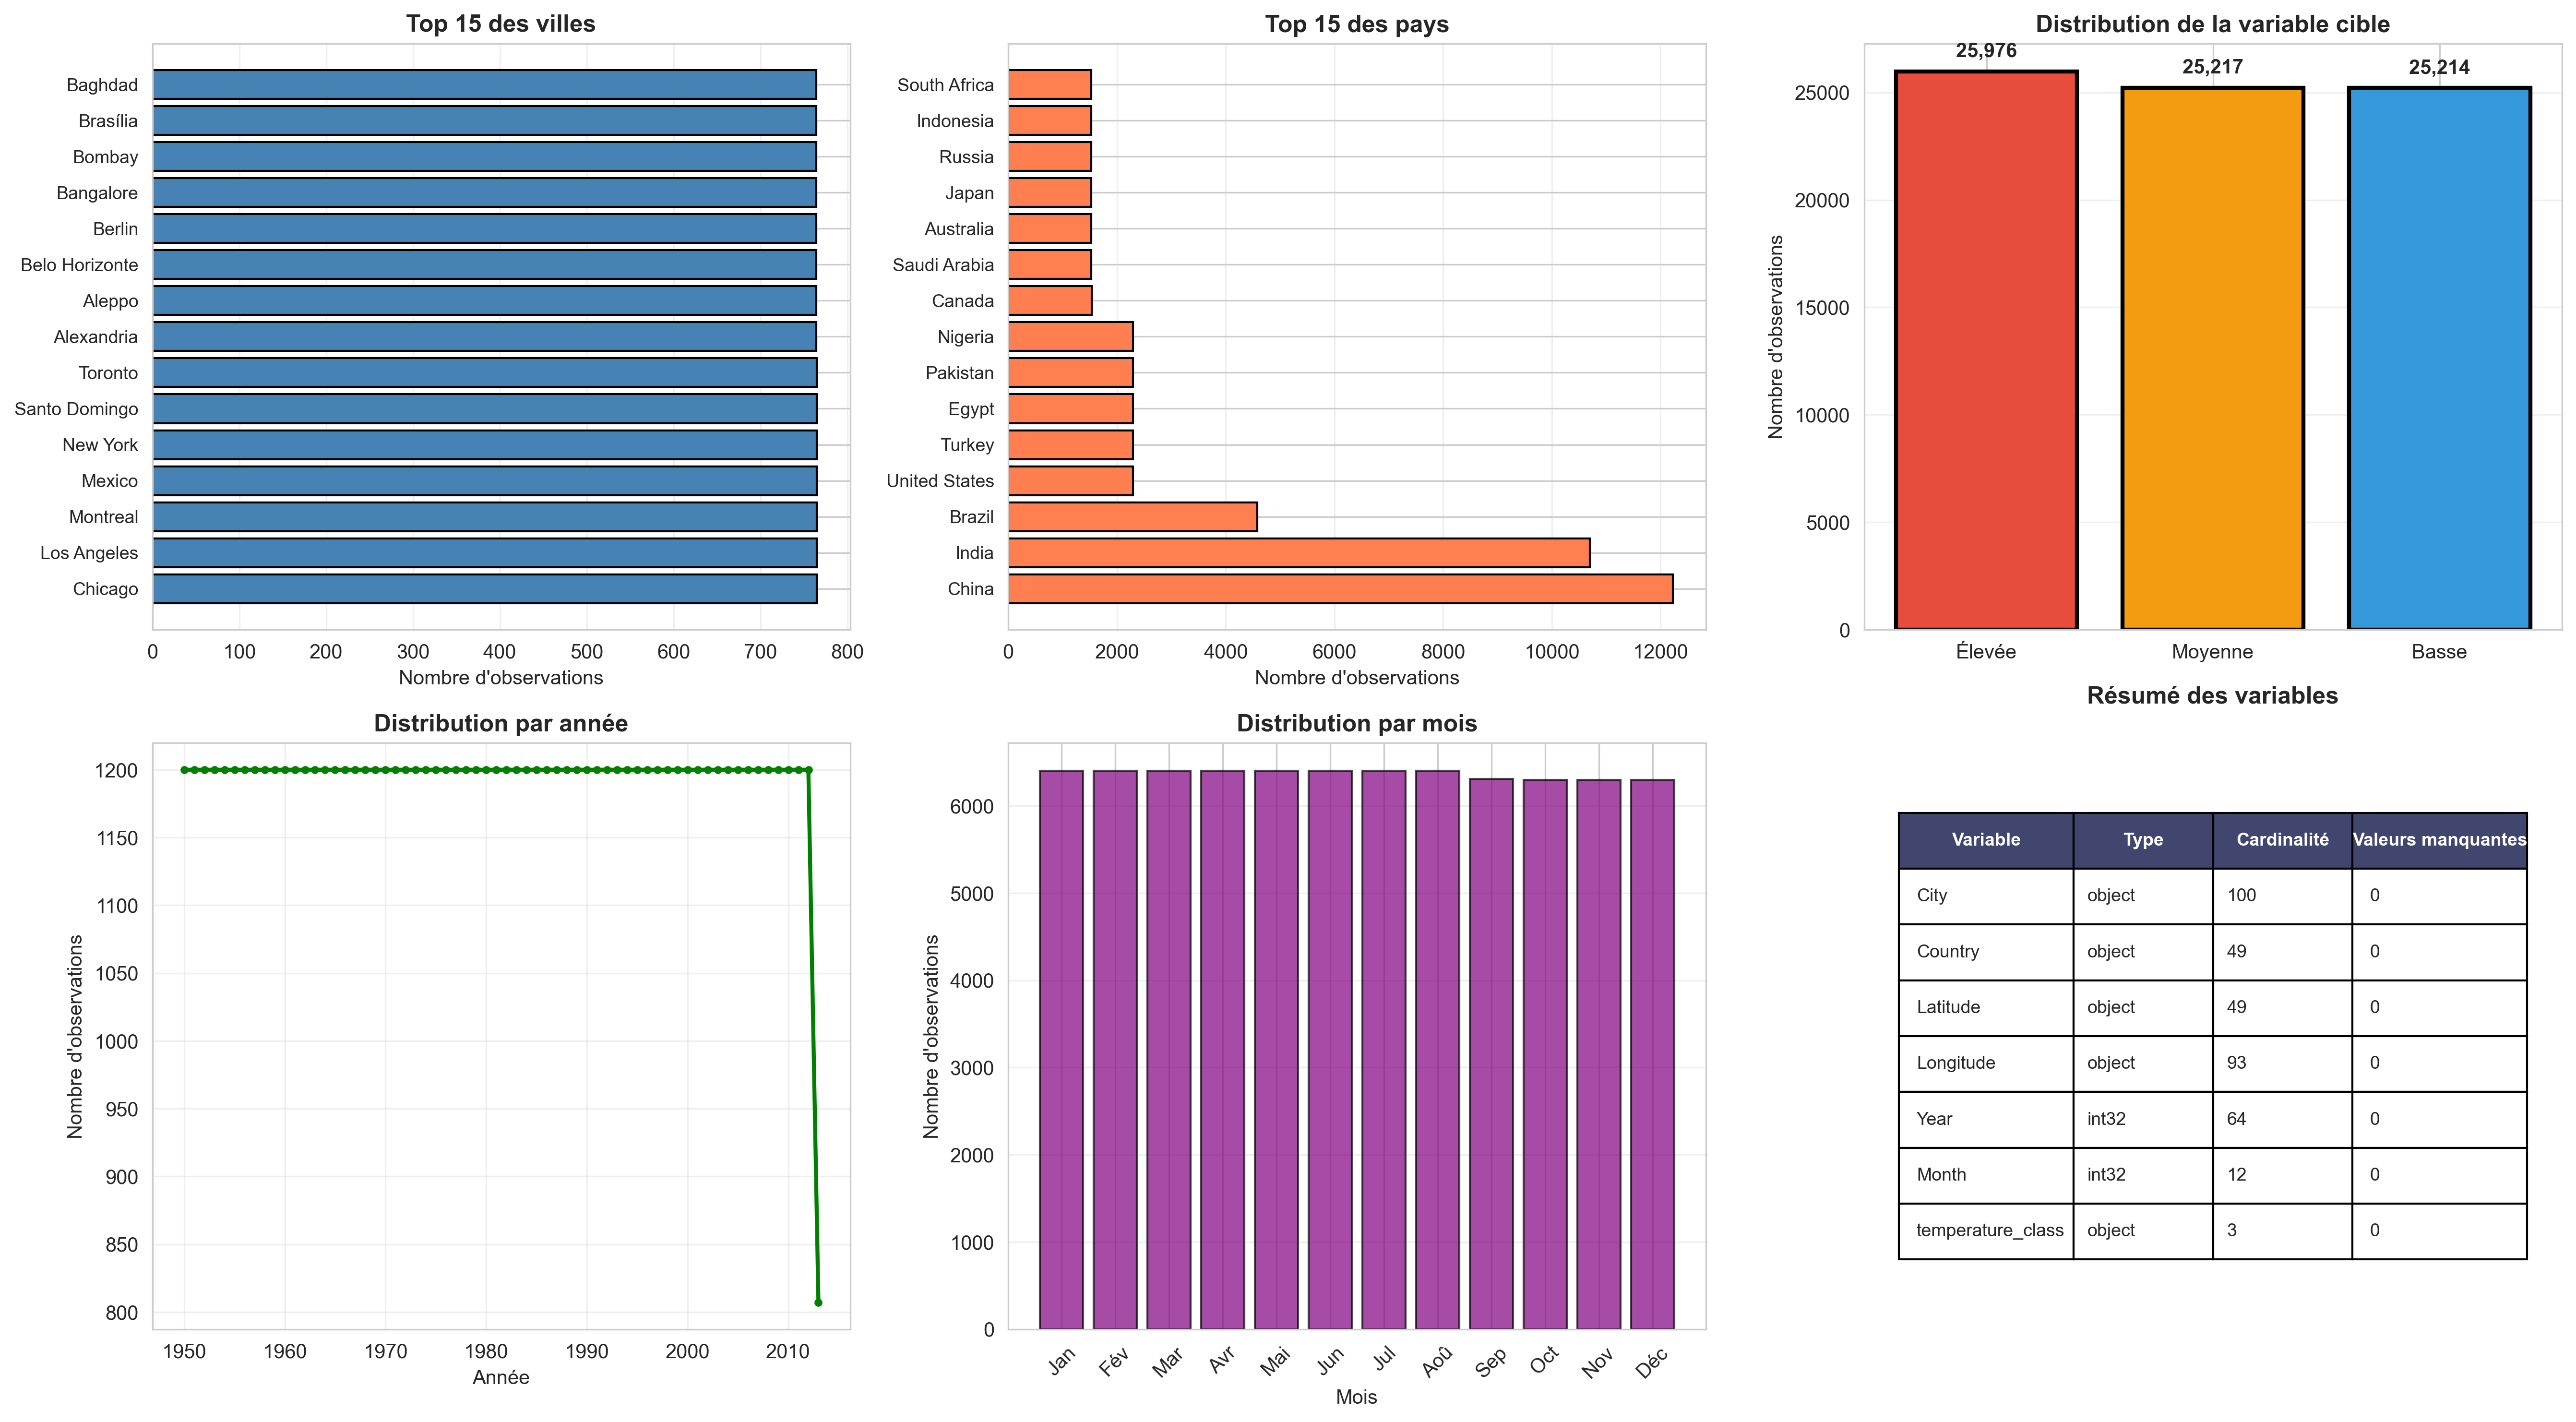
\includegraphics[width=0.88\textwidth]{step4_sipina_preparation.png}
\caption{Préparation Sipina (étape 4)}
\end{figure}

\section{Étape 5 -- Modélisation avec Sipina}
\subsection{Méthodologie}
Bien que Sipina soit l'outil recommandé, un arbre de décision a été construit avec scikit-learn pour : valider la préparation, identifier les variables importantes, et extraire des règles.

\subsection{Variables les plus importantes}
\begin{table}[H]
\centering
\footnotesize
\begin{tabular}{lcc}
\toprule
\textbf{Rang} & \textbf{Variable} & \textbf{Importance} \\
\midrule
1 & Month & 98,6\% \\
2 & Year & 1,4\% \\
\bottomrule
\end{tabular}
\caption{Variables les plus importantes}
\end{table}

\subsection{Règles de décision extraites}
\textbf{Règle 1 :} saisonnalité estivale (mois 6--8) $\Rightarrow$ \textit{Élevée}.

\textbf{Règle 2 :} saisonnalité hivernale (mois 12,1,2) $\Rightarrow$ \textit{Basse}.

\textbf{Règle 3 :} mois intermédiaires (printemps/automne) : l'année joue un rôle complémentaire.

\subsection{Performance du modèle}
\begin{itemize}
\item \textbf{Précision entraînement} : 46.0\%
\item \textbf{Précision test} : 45.7\%
\end{itemize}

\subsection{Interprétation métier globale}
\begin{enumerate}
\item \textbf{Saisonnalité dominante} : le mois est le facteur principal.
\item \textbf{Tendance temporelle} : l'année apporte un signal long terme.
\item \textbf{Applications} : urbanisme, assurance, planification énergétique.
\end{enumerate}

\begin{figure}[H]
\centering
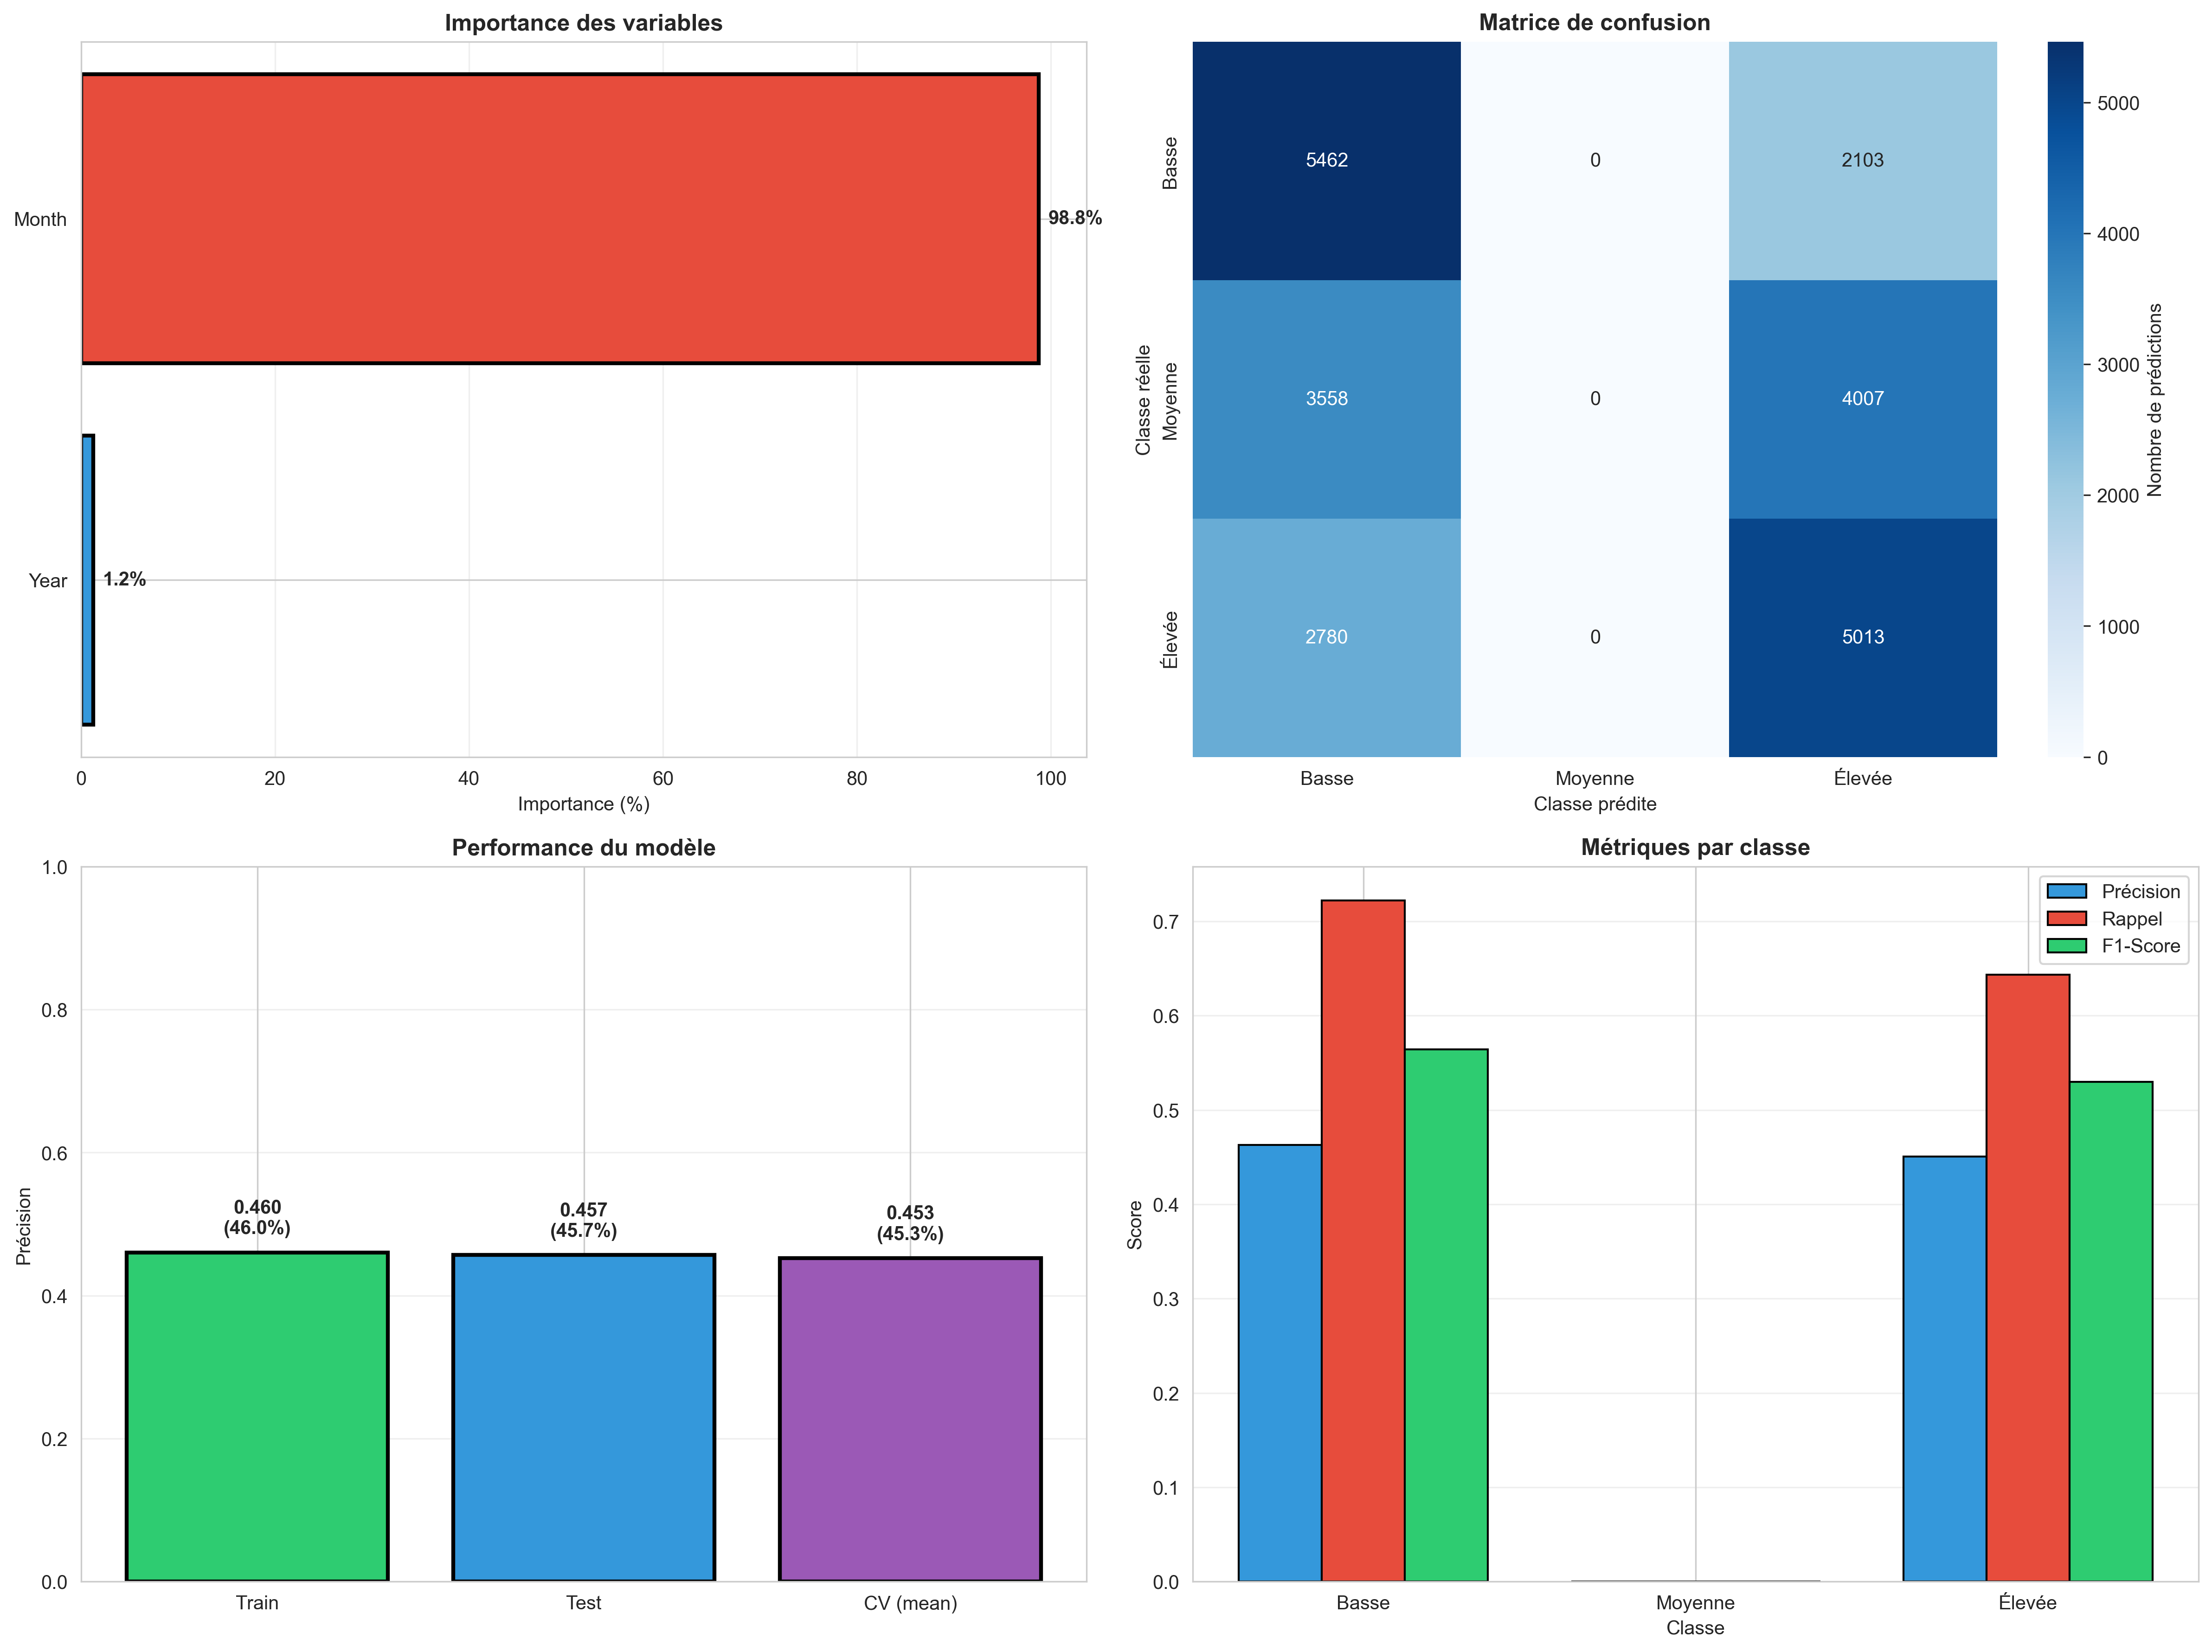
\includegraphics[width=0.90\textwidth]{step5_model_performance.png}
\caption{Modélisation (étape 5)}
\end{figure}

\section{Étape 6 -- Mise en perspective Big Data}
Dans ce projet, \textasciitilde{}76\,000 lignes sont traitées avec Pandas. En contexte industriel, les volumes seraient bien plus importants (données horaires, multi-sources, couverture élargie), rendant nécessaire un framework distribué.

\subsection{Pourquoi Spark ?}
\begin{itemize}
\item Calcul distribué et parallélisation.
\item Lecture/écriture partitionnée.
\item Agrégations et statistiques globales à grande échelle.
\end{itemize}

\subsection{Étapes bénéficiant le plus du distribué}
\begin{itemize}
\item Étape 2 : réduction et agrégation.
\item Étape 3 : calcul de quantiles et transformations.
\end{itemize}

\textbf{Principe clé :} \textit{\og Réduire avec Spark, analyser avec des outils spécialisés\fg{}}.

\section{Conclusion générale}
\subsection{Objectifs atteints}
\begin{itemize}
\item Réduction de \textasciitilde{}239k lignes à \textasciitilde{}76k lignes pertinentes.
\item Pipeline clair et reproductible.
\item Règles d'arbre interprétables.
\end{itemize}

\subsection{Perspectives d'amélioration}
\begin{itemize}
\item Conversion latitude/longitude en numérique.
\item Analyse par régions climatiques.
\item Étude du réchauffement local par ville.
\end{itemize}

\vspace{0.2cm}
\colorbox{boxcolor}{\parbox{0.96\textwidth}{\footnotesize\textbf{Reproductibilité :} exécuter \texttt{python main.py} pour régénérer les fichiers \texttt{dataset\_*.csv} et les figures dans \texttt{outputs/}.}}

\end{document}
